\selectlanguage{italian}
\graphicspath{ {img/2/} }
\chapter{Artificial Intelligence e Machine Learning}\label{cap:CenniAIeML}
\thispagestyle{empty} %Elimina il numero della prima pagina del capitolo.
\newpage

\section{L'\acf{AI}}
\vspace{8mm}
Nella sua accezione più semplice, l'intelligenza artificiale (AI) si riferisce a sistemi o macchine che imitano l'intelligenza umana per eseguire determinate attività e che sono in grado di migliorare continuamente in base alle informazioni raccolte. L'intelligenza artificiale si manifesta in varie forme. Di seguito sono riportati alcuni esempi:

\begin{itemize}
    \item I \textbf{chatbot} utilizzano l'intelligenza artificiale per comprendere più rapidamente i problemi dei clienti e fornire risposte più efficaci. 
    \item Gli \textbf{assistenti intelligenti} utilizzano l'intelligenza artificiale per analizzare le informazioni importanti provenienti da una grande quantità di dati testuali per migliorare la pianificazione.
    \item I \textbf{motori di raccomandazione} possono fornire consigli automatici per programmi TV in base alle abitudini televisive degli utenti.
\end{itemize}

L'intelligenza artificiale fornisce i processi e le capacità per potenziare al massimo la riflessione e l'analisi dei dati. Lo scopo dell'intelligenza artificiale è quello di migliorare in modo significativo le abilità e le attività degli esseri umani. Per questo motivo, è una risorsa molto preziosa per le aziende.

Il termine "intelligenza artificiale" viene utilizzato in modo generico per indicare le applicazioni che eseguono attività complesse che in passato richiedevano l'intervento umano, come comunicare con i clienti online o giocare a scacchi. Il termine viene spesso utilizzato in maniera interscambiabile con i termini \emph{Machine Learning} e \emph{Deep Learning}. Tuttavia, ci sono delle differenze: ad esempio, il Machine Learning è incentrato sulla creazione di sistemi che apprendono o migliorano le loro performance in base ai dati che utilizzano. È importante notare che, sebbene il Machine Learning sia sempre definibile come intelligenza artificiale, l'intelligenza artificiale non è sempre equivalente al Machine Learning.

Per sfruttare appieno il valore dell'intelligenza artificiale, molte aziende stanno investendo in modo significativo in team addetti al data science. \emph{Data science} è un settore interdisciplinare che utilizza metodi scientifici per estrarre valore dai dati e combina le competenze di settori quali la statistica e l'informatica con le conoscenze aziendali per analizzare i dati raccolti da più fonti.

Il fondamento su cui poggia l'intelligenza artificiale, ovvero la capacità di replicare e superare il modo in cui gli umani percepiscono e reagiscono al mondo, sta diventando rapidamente la pietra miliare dell'innovazione. Grazie al Machine Learning, che riconosce gli schemi nei dati e permette di fare previsioni, l'intelligenza artificiale potrà raggiungere notevoli traguardi.

La tecnologia AI sta migliorando le performance e la produttività delle aziende grazie all'automazione dei processi o delle attività che in passato richiedevano l'intervento umano. Inoltre, l'intelligenza artificiale può sfruttare i dati a un livello che nessun essere umano potrebbe mai raggiungere.
\cite{introAI}

\newpage
\section{Machine Learning}
\vspace{8mm}

Il Machine Learning è un sottoinsieme dell'intelligenza artificiale (AI) che si occupa di creare sistemi che apprendono o migliorano le performance in base ai dati che utilizzano. Intelligenza artificiale è un termine generico e si riferisce a sistemi o macchine che imitano l'intelligenza umana. I termini Machine Learning e Intelligenza Artificiale vengono spesso utilizzati insieme e in modo interscambiabile, ma non hanno lo stesso significato. Un'importante distinzione è che sebbene tutto ciò che riguarda il Machine Learning rientra nell'intelligenza artificiale, l'intelligenza artificiale non include solo il Machine Learning.

Attualmente, il Machine Learning è utilizzato in qualsiasi contesto. Quando interagiamo con le banche, acquistiamo online o utilizziamo i social media, vengono utilizzati algoritmi di Machine Learning per rendere la nostra esperienza efficiente, facile e sicura. Il Machine Learning e le tecnologie ad esso associate si stanno sviluppando rapidamente e le loro funzionalità sono in continua evoluzione.

Gli algoritmi sono i motori che alimentano il Machine Learning. I due tipi principali di algoritmi di ML attualmente utilizzati sono gli \emph{algoritmi supervisionati} e gli \emph{algoritmi non supervisionati}. La differenza tra questi due tipi viene definita dal modo in cui ciascun algoritmo apprende i dati per fare previsioni.

\newpage\textbf{Machine Learning supervisionato}\newline	
Gli algoritmi di Machine Learning supervisionato sono i più utilizzati. Con questo modello, un Data Scientist agisce da guida e insegna all'algoritmo i risultati da generare. Esattamente come un bambino impara a identificare i frutti memorizzandoli in un libro illustrato, nel Machine Learning supervisionato l'algoritmo apprende da un set di dati già etichettato e con un output predefinito.

Esempi di algoritmi di Machine Learning supervisionato sono gli algoritmi di regressione lineare e logistica, di classificazione multiclasse e le macchine a vettori di supporto.\newline

\textbf{Machine Learning non supervisionato}\newline
Il Machine Learning non supervisionato utilizza un approccio più indipendente, in cui un computer impara a identificare processi e schemi complessi senza la guida attenta e costante di una persona. Il Machine Learning non supervisionato implica una formazione basata su dati privi di etichette e per i quali non è stato definito un output specifico.

Utilizzando ancora una volta la precedente analogia, il Machine Learning non supervisionato è simile a un bambino che impara a identificare i frutti osservando i colori e gli schemi, anziché memorizzando i nomi con l'aiuto di un insegnante. Il bambino cercherà le somiglianze tra le immagini e le suddividerà in gruppi, assegnando a ciascun gruppo la nuova etichetta corrispondente.

Esempi di algoritmi di Machine Learning non supervisionato
sono gli algoritmi di clustering k-means, l'analisi di componenti principali e indipendenti e le regole di associazione.

Un'altra straordinaria caratteristica del Machine Learning è la sua capacità predittiva. In passato, le decisioni aziendali venivano spesso prese sulla base di risultati storici. Oggi, il Machine Learning utilizza analisi dei dati avanzate per eseguire previsioni. Le organizzazioni possono prendere decisioni proattive e lungimiranti anziché fare affidamento sui dati passati.

Ad esempio, la manutenzione predittiva può consentire ai produttori, alle aziende energetiche e ad altri settori di prendere l'iniziativa e verificare che le loro operazioni rimangano affidabili e ottimizzate. In un giacimento petrolifero con centinaia di trivelle in funzione, i modelli di Machine Learning possono individuare apparecchiature a rischio di malfunzionamento a breve termine e quindi avvisare i team di manutenzione in anticipo. Questo approccio non solo ottimizza la produttività, ma aumenta le performance delle risorse, dei tempi di attività e la durata delle apparecchiature. Può inoltre ridurre al minimo i rischi per i lavoratori.
\cite{introML}

\newpage
\section{Data, Datasets e Preprocessing}
\vspace{8mm}
\subsection{Data}
I metodi di \acf{ML} apprendono dagli esempi. È importante avere una buona conoscenza dei dati di input e delle varie terminologie utilizzate nella descrizione dei dati. Di seguito è riportata la terminologia fondamentale e necessaria per comprendere al meglio i dati utilizzati per algoritmi di Machine Learning.

\begin{itemize}
    \item \textbf{Istanza}: Una singola riga di dati è chiamata istanza. È un'osservazione dal dominio
    \item \textbf{Feature}: Una singola colonna di dati è chiamata feature. È una componente di un'osservazione ed è anche chiamata attributo di un'istanza di dati. Alcune feature possono essere input per un modello, altre possono essere output o feature da prevedere.
    \item \textbf{Data Type}: Le feature hanno un tipo di dati. Possono essere reali o interi o avere un valore categorico o ordinale. Possono essere stringhe, date, orari e tipi più complessi, ma in genere vengono ridotti a valori reali o categorici quando si lavora con i metodi di Machine Learning tradizionali.
    \item \textbf{Dataset}: Una raccolta di istanze è un set di dati. Quando si lavora con metodi di Machine Learning sono necessari alcuni set di dati per scopi diversi.
\end{itemize} 

In genere, per ottenere un modello di Machine Learning, in particolare nel caso del software prodotto, ossia un modello  di classificazione binaria a partire da immagini, viene utilizzato un Dataset contenente sia immagini specifiche, riguardanti il tipo di oggetto da classificare, che immagini non specifiche in cui non è presente l'oggetto da classificare. Questi dati sono quindi accompagnati da etichette o \emph{label} il cui scopo è quello di indicare \emph{l'output corretto} al modello, durante la fase di training.
\begin{figure}[h!]
	\centering
	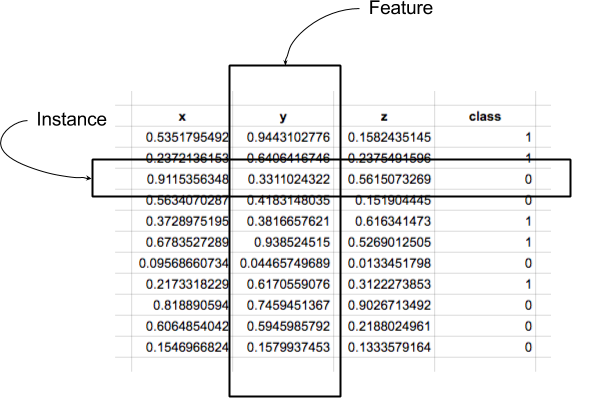
\includegraphics[width=120mm]{img/2/ds_1_1.png}
	\caption{\fontsize{10px}{0mm}\selectfont Istanze e Feature\label{fig:ds_1_1}}
\end{figure}\newline
\subsection{Dataset}
I Dataset, come descritto precedentemente, sono una raccolta di istanze (righe di dati). I Dataset possono essere strutturati o non strutturati. Si parla di \emph{Dataset strutturato} quando i dati in esso contenuti sono conservati in database, organizzati secondo schemi e tabelle rigide. Si parla di \emph{Dataset non strutturato} quando i dati sono conservati senza alcuno schema particolare. Nel caso dei Dataset non strutturati, i sistemi di gestione di dati utilizzabili sono quelli basati sul modello dell’information retrieval.
Alcuni esempi di Dataset strutturati sono i Dataset organizzati secondo strutture quali \ac{CSV}, \ac{TSV}, \ac{JSON}, \ac{XML}, \ac{HTML} e \ac{SQL}.
Nel caso del software sviluppato, i dati sono \textit{non strutturati} poichè si ha a che fare con immagini non conservate in alcun tipo di struttura e senza una particolare organizzazione.

\subsection{Preprocessing}
Quando si affronta un problema di Machine Learning il primo passo consiste nel predisporre di un buon Training set(dataset utilizzato unicamente per la fase di training) a partire dai dataset disponibili in maniera tale da costruire un modello accurato.

É quindi necessaria un’analisi preliminare il cui scopo è quello di evidenziare eventuali criticità e ristrutturare i dati in modo da eliminarne criticità individuate.

Un esempio pratico riguarda la verifica della presenza di valori nulli rispetto alle feature. Dal momento che questi possono compromettere la qualità del modello occorre eliminarli. É possibile procedere in due modi:

\begin{enumerate}
    \item Rimuovere gli esempi con valori 
    \item Sostituire i valori nulli con altri calcolati in maniera opportuna (media della relativa colonna)
\end{enumerate}
Nei problemi di classificazione si ha spesso a che fare con categorie non numeriche che possono creare problemi. Occorre mappare opportunamente le classi con valori ordinali.

Nel caso di valori numerici è abbastanza comune ricorrere alla normalizzazione e alla standardizzazione dei dati.
\newpage
La normalizzazione consente di mappare i valori nell’intervallo [0,1] e si ottiene trasformando ciascun datapoint $x_i$ in

$$x_i = \frac{x_i-x_{min}}{x_{max} - x_{min}}$$

dove $x_{min}$ e $x_{max}$ sono rispettivamente il minimo e il massimo dell’intervallo di partenza.

La standardizzazione punta a centrare i dati intorno allo 0 e a scalarli tenendo presente la deviazione standard.

Ciascun $x_i$ diventa

$$x_i = \frac{x_i-\mu}{\sigma}$$

dove $\mu$ è la media e $\sigma$ è la deviazione standard.

Naturalmente queste trasformazioni agiscono solo sull’intervallo dei dati ma non sulla loro distribuzione che resta inalterata.\cite{preprocessing}\newpage

\section{Problematiche legate alla fase di Training}

Quando si parla di Training si intende "adattamento" ai dati o "apprendimento" dai dati. Durante questa fase il modello inizia ad apprendere a partire dai dati forniti. Questo passaggio è fondamentale poiché l'output finale (o previsione) del modello si baserà sulla capacità del modello di acquisire i pattern dei dati di addestramento.

Un training improprio può portare a un drastico degrado delle prestazioni del modello al momento dell'implementazione. Visti ad alto livello, esistono due tipi principali di risultati della formazione impropria: \emph{underfitting} e \emph{overfitting}.

\subsection{Underfitting}
Quando la complessità del modello è troppo ridotta perché esso apprenda i dati forniti come input, il modello si dice sia in "Underfit". In altre parole, un modello eccessivamente semplice non riesce ad apprendere le tendenze sottostanti ai dati in input. Tale risultato è causato da un modello con bassa varianza\footnote{La varianza di una variabile statistica è una funzione che fornisce una misura della variabilità dei valori assunti dalla variabile stessa} e bias elevato.\newline
Visualizzare graficamente un modello in underfitting può essere di aiuto nel determinare se il modello non fornisce dati adeguati durante il training.
Il seguente grafico mostra un modello il cui scopo è quello di \emph{classificare} i dati nelle classi \textit{Croce} e \textit{Cerchio}

\begin{figure}[h!]
	\centering
	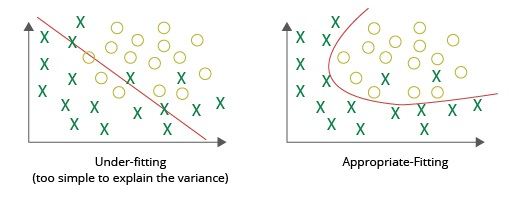
\includegraphics[width=120mm]{img/2/underover_1_1}
	\caption{\fontsize{10px}{0mm}\selectfont Underfitting in un task di classificazione\label{fig:underover_1_1}}
\end{figure}
\newpage
\subsection{Overfitting}
Quando la complessità del modello è troppo elevata rispetto ai dati che sta cercando di apprendere, il modello si dice sia in "Overfit". In altre parole, aumentando la complessità del modello, esso tende ad adattarsi ai noisy data\footnote{Dati con un'abbondanza di informazioni addizionali. Dati corrotti o disturbati.} presente e agli outliers\footnote{Dati che deviano in maniera significativa rispetto al resto dei dati, possono essere causati da errori di misurazione.} presenti nei dati. Il modello ha appreso troppo e quindi non è più in grado di generalizzare.
Tale risultato è causato da un modello con alta varianza e basso bias.\cite{underfitoverfit}\newline
Di seguito è mostrato un modello in overfit utilizzando il precedente esempio.

\begin{figure}[h!]
	\centering
	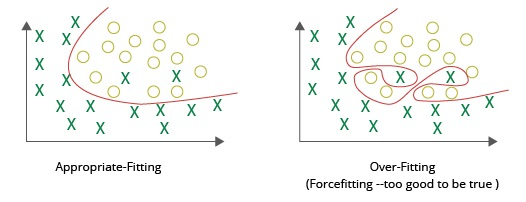
\includegraphics[width=120mm]{img/2/underover_1_2}
	\caption{\fontsize{10px}{0mm}\selectfont Overfitting in un task di classificazione\label{fig:underover_1_2}}
\end{figure}
\newpage
